\documentclass[11pt,a4paper]{article}

%% ── Packages ─────────────────────────────────────────────────────────────────
\usepackage[top=2.2cm,bottom=2.2cm,left=2cm,right=2cm]{geometry}
\usepackage[T1]{fontenc}
\usepackage[utf8]{inputenc}
\usepackage{lmodern}
\usepackage{microtype}
\usepackage{graphicx}
\usepackage{float}
\usepackage{caption}
\usepackage{enumitem}
\usepackage{booktabs}
\usepackage{array}
\usepackage{tabularx}
\usepackage{xcolor}
\usepackage{titlesec}
\usepackage{fancyhdr}
\usepackage[hidelinks]{hyperref}
\usepackage{parskip}

%% ── Colours ──────────────────────────────────────────────────────────────────
\definecolor{accent}{RGB}{37,99,235}
\definecolor{seccolor}{RGB}{30,30,30}
\definecolor{muted}{RGB}{140,133,124}
\definecolor{border}{RGB}{227,221,211}

%% ── Section styling ──────────────────────────────────────────────────────────
\titleformat{\section}{\large\bfseries\color{seccolor}}{}{0em}{}[\color{border}\titlerule]
\titleformat{\subsection}{\normalsize\bfseries}{}{0em}{}
\titlespacing{\section}{0pt}{18pt}{8pt}
\titlespacing{\subsection}{0pt}{12pt}{4pt}

%% ── Header / Footer ──────────────────────────────────────────────────────────
\pagestyle{fancy}\fancyhf{}
\renewcommand{\headrulewidth}{0.4pt}
\fancyhead[L]{\small\textcolor{muted}{CS310 — Mobile Application Development}}
\fancyhead[R]{\small\textcolor{muted}{ChefInPocket · UI Implementation Report}}
\fancyfoot[C]{\small\thepage}

%% ── List spacing ─────────────────────────────────────────────────────────────
\setlist[itemize]{noitemsep,topsep=3pt,leftmargin=1.4em}
\setlist[enumerate]{noitemsep,topsep=3pt,leftmargin=1.4em}
\captionsetup{font=small,labelfont=bf,skip=4pt}

%% ── Layout helpers ───────────────────────────────────────────────────────────
\newcommand{\sblock}[4]{%
  \begin{minipage}[t]{0.30\textwidth}
    \centering
    \includegraphics[width=0.88\linewidth]{#1}\\[5pt]
    {\small\bfseries Screen #2 — #3}\\[5pt]
    {\footnotesize #4}
  \end{minipage}}

\newenvironment{sidebyside}[3]{%
  \noindent
  \begin{minipage}[t]{0.34\textwidth}
    \vspace{0pt}%
    \centering
    \includegraphics[width=0.80\linewidth]{#1}\\[5pt]
    {\small\bfseries Screen #2 — #3}
  \end{minipage}%
  \hfill
  \begin{minipage}[t]{0.62\textwidth}
    \vspace{0pt}%
}{%
  \end{minipage}
  \medskip}

%% ─────────────────────────────────────────────────────────────────────────────
\begin{document}

%% ══════════════════════════════════════════════════════════════
%% COVER BLOCK
%% ══════════════════════════════════════════════════════════════
\begin{center}
  {\large\bfseries CS310 — Mobile Application Development}\\[4pt]
  {\large [Spring 2025--2026] Project Step 3: UI Implementation}\\[4pt]
  {\large Group 03 · \textbf{ChefInPocket} \quad
    \href{https://github.com/mesely/ChefInPocket.git}{\textcolor{accent}{(GitHub Repository)}}}
\end{center}

\medskip
\noindent\textcolor{border}{\rule{\linewidth}{0.4pt}}
\medskip

%% ══════════════════════════════════════════════════════════════
\section{Application Overview}

\textbf{ChefInPocket} is a mobile cooking-assistant application built with Flutter that guides users from ingredient selection through step-by-step cooking, with AI support at every stage. In this step, the wireframes designed in Step~2 have been fully transformed into \textbf{20 functional Flutter screens} connected by a clean navigation system, backed by a live REST API, and polished with custom typography and a consistent design language.

\subsection*{Core Features Implemented}
\begin{itemize}
  \item \textbf{Recipe Discovery} — Browse by cuisine (6 categories) or search by name with live autocomplete suggestions.
  \item \textbf{Ingredient-Based Matching} — Multi-select ingredient picker that calls the API and returns matching recipes instantly.
  \item \textbf{Serving Scale} — Stepper widget recalculates all ingredient amounts in real time via API.
  \item \textbf{AI Chef Chat} — Full-screen conversational assistant with recipe context, left/right chat bubbles, and scroll-to-latest behavior.
  \item \textbf{Grocery List} — Item cards with dynamic deletion; quick-add bottom sheet with 12 ingredient chips.
  \item \textbf{Community \& Social} — Feed with Q\&A posting, bookmarking, and user profile browsing.
  \item \textbf{Saved Recipes} — Bookmarked recipes stored via API, removable with a single tap.
  \item \textbf{My Recipes / Add Recipe} — Users can publish and view their own community posts.
  \item \textbf{Customize Ingredients} — Replace or remove elements from a recipe without breaking proportions.
  \item \textbf{Cooking Steps} — All steps displayed as numbered cards; Mark as Done navigates back to Home.
\end{itemize}

%% ══════════════════════════════════════════════════════════════
\section{Team Contribution}

\begin{center}
\begin{tabularx}{0.97\textwidth}{llX}
\toprule
\textbf{Team Member} & \textbf{Student ID} & \textbf{Screens Implemented} \\
\midrule
Emir Keskin        & 31020 & Onboarding, Browse Cuisine, Recipe Detail, Ingredient Picker \\
Cem Özkul          & 34183 & Login, Register, Recipe Results, Add Recipe \\
Nilsu Saraçlar     & 34210 & Home, Serving Scale, Saved Recipes \\
Mehmet Selman Yılmaz & 31158 & AI Chat, Cooking Steps, My Recipes, Ask Q\&A \\
Doğa Atılğan       & 34450 & Grocery List, Community, Customize Ingredients \\
Bora Demirkol      & 32361 & Profile, User Profile, Navigation Architecture \& Routing \\
\bottomrule
\end{tabularx}
\end{center}

All members contributed equally to integration, cross-screen consistency, and the overall app structure.

%% ══════════════════════════════════════════════════════════════
\newpage
\section{Navigation Flow}

All navigation in ChefInPocket uses Flutter's named route system. The \texttt{initialRoute} is set to \texttt{AppRoutes.onboarding} in \texttt{MaterialApp}. The application flow is structured into five logical branches:

\begin{enumerate}
  \item \textbf{Access Branch:} Onboarding $\rightarrow$ Register \emph{or} Login $\rightarrow$ Home.\\
        Login and Register use \texttt{pushNamedAndRemoveUntil} so the back button cannot return to auth screens after sign-in.
  \item \textbf{Discovery Branch:} Home $\rightarrow$ Browse Cuisine $\rightarrow$ Ingredient Picker $\rightarrow$ Recipe Results $\rightarrow$ Recipe Detail.
  \item \textbf{Recipe Tool Branch:} Recipe Detail $\rightarrow$ Serving Scale \emph{/} Customize Ingredients \emph{/} Cooking Steps \emph{/} AI Chat.
  \item \textbf{Social Branch:} Community $\rightarrow$ Ask Q\&A \emph{or} User Profile; Profile $\rightarrow$ Saved Recipes \emph{/} My Recipes \emph{/} Add Recipe.
  \item \textbf{Main Tab Branch:} Bottom navigation bar (Home, Community, Grocery List, Profile) uses \texttt{pushReplacementNamed} to swap root screens without stacking them.
\end{enumerate}

\subsection*{Named Routes Defined in \texttt{lib/routes/app\_routes.dart}}

\begin{center}
\begin{tabularx}{0.96\textwidth}{lX}
\toprule
\textbf{Route Constant} & \textbf{Path / Screen} \\
\midrule
\texttt{AppRoutes.onboarding}           & \texttt{/} — OnboardingScreen \\
\texttt{AppRoutes.login}                & \texttt{/login} — LoginScreen \\
\texttt{AppRoutes.register}             & \texttt{/register} — RegisterScreen \\
\texttt{AppRoutes.home}                 & \texttt{/home} — HomeScreen \\
\texttt{AppRoutes.community}            & \texttt{/community} — CommunityScreen \\
\texttt{AppRoutes.groceryList}          & \texttt{/grocery-list} — GroceryListScreen \\
\texttt{AppRoutes.profile}              & \texttt{/profile} — ProfileScreen \\
\texttt{AppRoutes.recipeDetail}         & \texttt{/recipe-detail} — RecipeDetailScreen \\
\texttt{AppRoutes.cookingSteps}         & \texttt{/cooking-steps} — CookingStepsScreen \\
\texttt{AppRoutes.recipeResults}        & \texttt{/recipe-results} — RecipeResultsScreen \\
\texttt{AppRoutes.ingredientPicker}     & \texttt{/ingredient-picker} — IngredientPickerScreen \\
\texttt{AppRoutes.savedRecipes}         & \texttt{/saved-recipes} — SavedRecipesScreen \\
\texttt{AppRoutes.browseCuisine}        & \texttt{/browse-cuisine} — BrowseCuisineScreen \\
\texttt{AppRoutes.servingScale}         & \texttt{/serving-scale} — ServingScaleScreen \\
\texttt{AppRoutes.customizeIngredients} & \texttt{/customize-ingredients} — CustomizeIngredientsScreen \\
\texttt{AppRoutes.aiChat}               & \texttt{/ai-chat} — AiChatScreen \\
\texttt{AppRoutes.addRecipe}            & \texttt{/add-recipe} — AddRecipeScreen \\
\texttt{AppRoutes.myRecipes}            & \texttt{/my-recipes} — MyRecipesScreen \\
\texttt{AppRoutes.askQA}                & \texttt{/ask-qa} — AskQAScreen \\
\texttt{AppRoutes.userProfile}          & \texttt{/user-profile} — UserProfileScreen \\
\bottomrule
\end{tabularx}
\end{center}

%% ══════════════════════════════════════════════════════════════
\newpage
\section{Implemented Screens}

%% ── 1. AUTH FLOW ─────────────────────────────────────────────────────────────
\subsection{Authentication Flow}

\medskip\noindent
\sblock{screenshots/onboarding.PNG}{1}{Onboarding}{%
  Initial entry point. Displays the app logo, app name, a short tagline, and two action buttons: \emph{Get Started} (Register) and \emph{Log In}. Vertically centred layout with \texttt{SafeArea} and \texttt{SingleChildScrollView}.}
\hfill
\sblock{screenshots/register.PNG}{2}{Register \textnormal{\tiny{(Input Form)}}}{%
  Account creation form with full name, email, password, and confirm password fields. Validates all four inputs; shows inline errors and displays a success \texttt{AlertDialog} on completion.}
\hfill
\sblock{screenshots/login_empty.PNG}{3}{Login \textnormal{\tiny{(Input Form)}}}{%
  Returning-user form with email and password fields. Pre-filled with demo credentials for testing. Includes a Log~In / Register segmented toggle at the top.}

\medskip\noindent
\begin{minipage}[t]{0.47\textwidth}
  \centering
  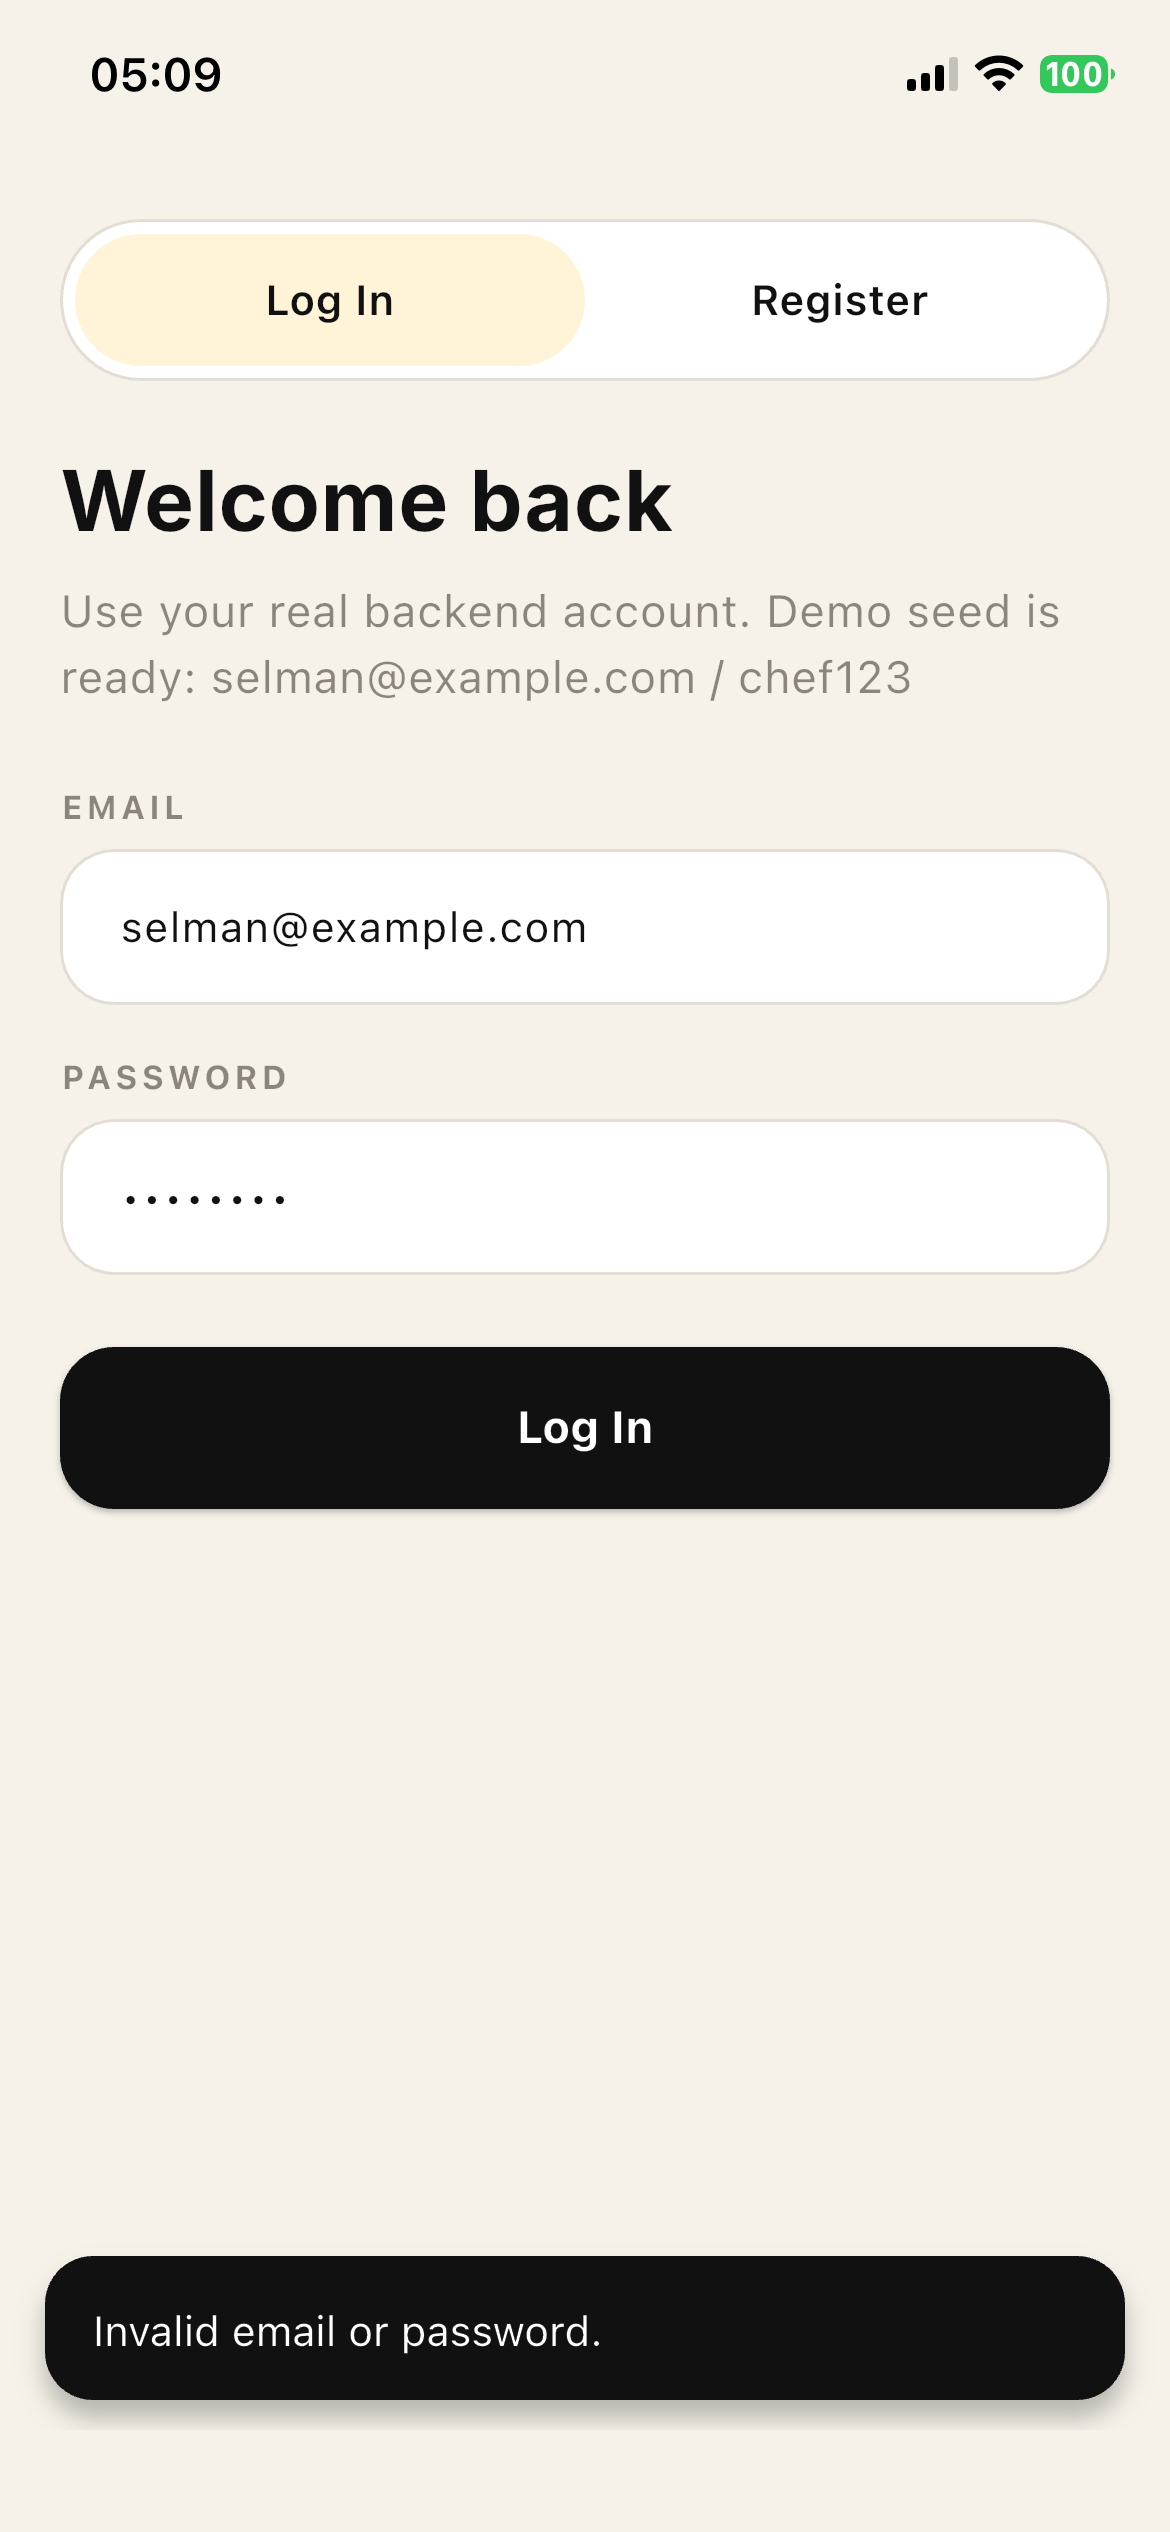
\includegraphics[width=0.52\linewidth]{screenshots/login_failed.PNG}\\[4pt]
  {\small\bfseries Login — Validation Error}\\[4pt]
  {\footnotesize Inline red error messages appear below each invalid field without leaving the screen. Both the email format and password length are validated before the API call is made.}
\end{minipage}
\hfill
\begin{minipage}[t]{0.47\textwidth}
  \centering
  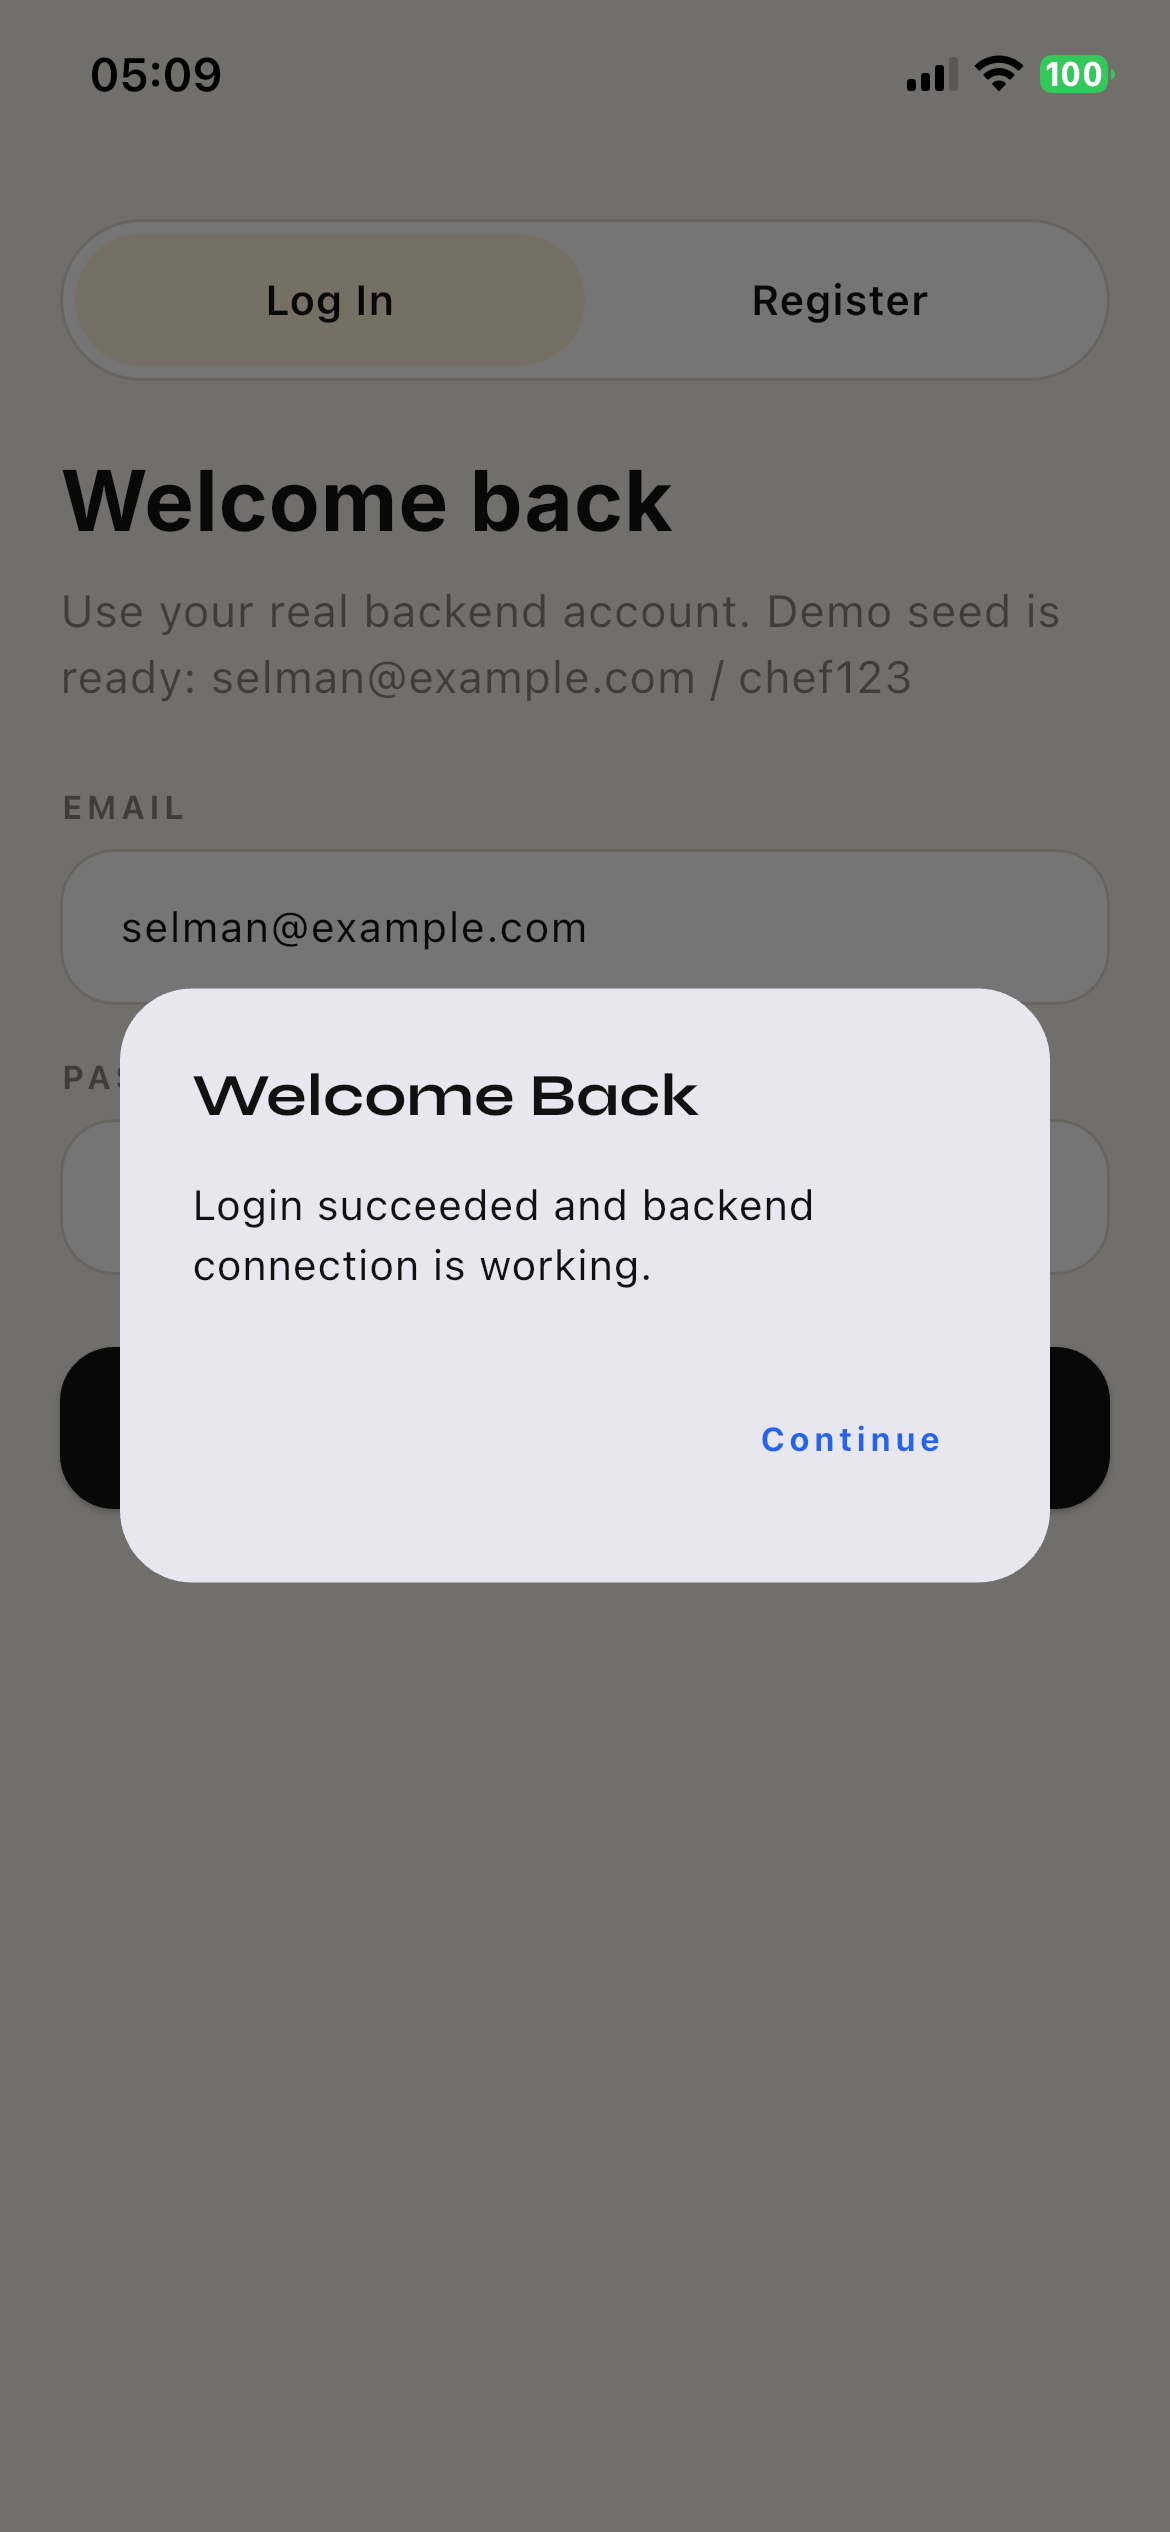
\includegraphics[width=0.52\linewidth]{screenshots/login_succesfull.PNG}\\[4pt]
  {\small\bfseries Login — Success AlertDialog}\\[4pt]
  {\footnotesize On a successful API login, \texttt{showSuccessDialog()} renders an \texttt{AlertDialog} with title \emph{Welcome Back} and a Continue button that clears the navigation stack and pushes Home.}
\end{minipage}

\medskip

%% ── 2. HOME ──────────────────────────────────────────────────────────────────
\subsection{Home Screen}

\noindent
\begin{minipage}[c]{0.34\textwidth}
  \centering
  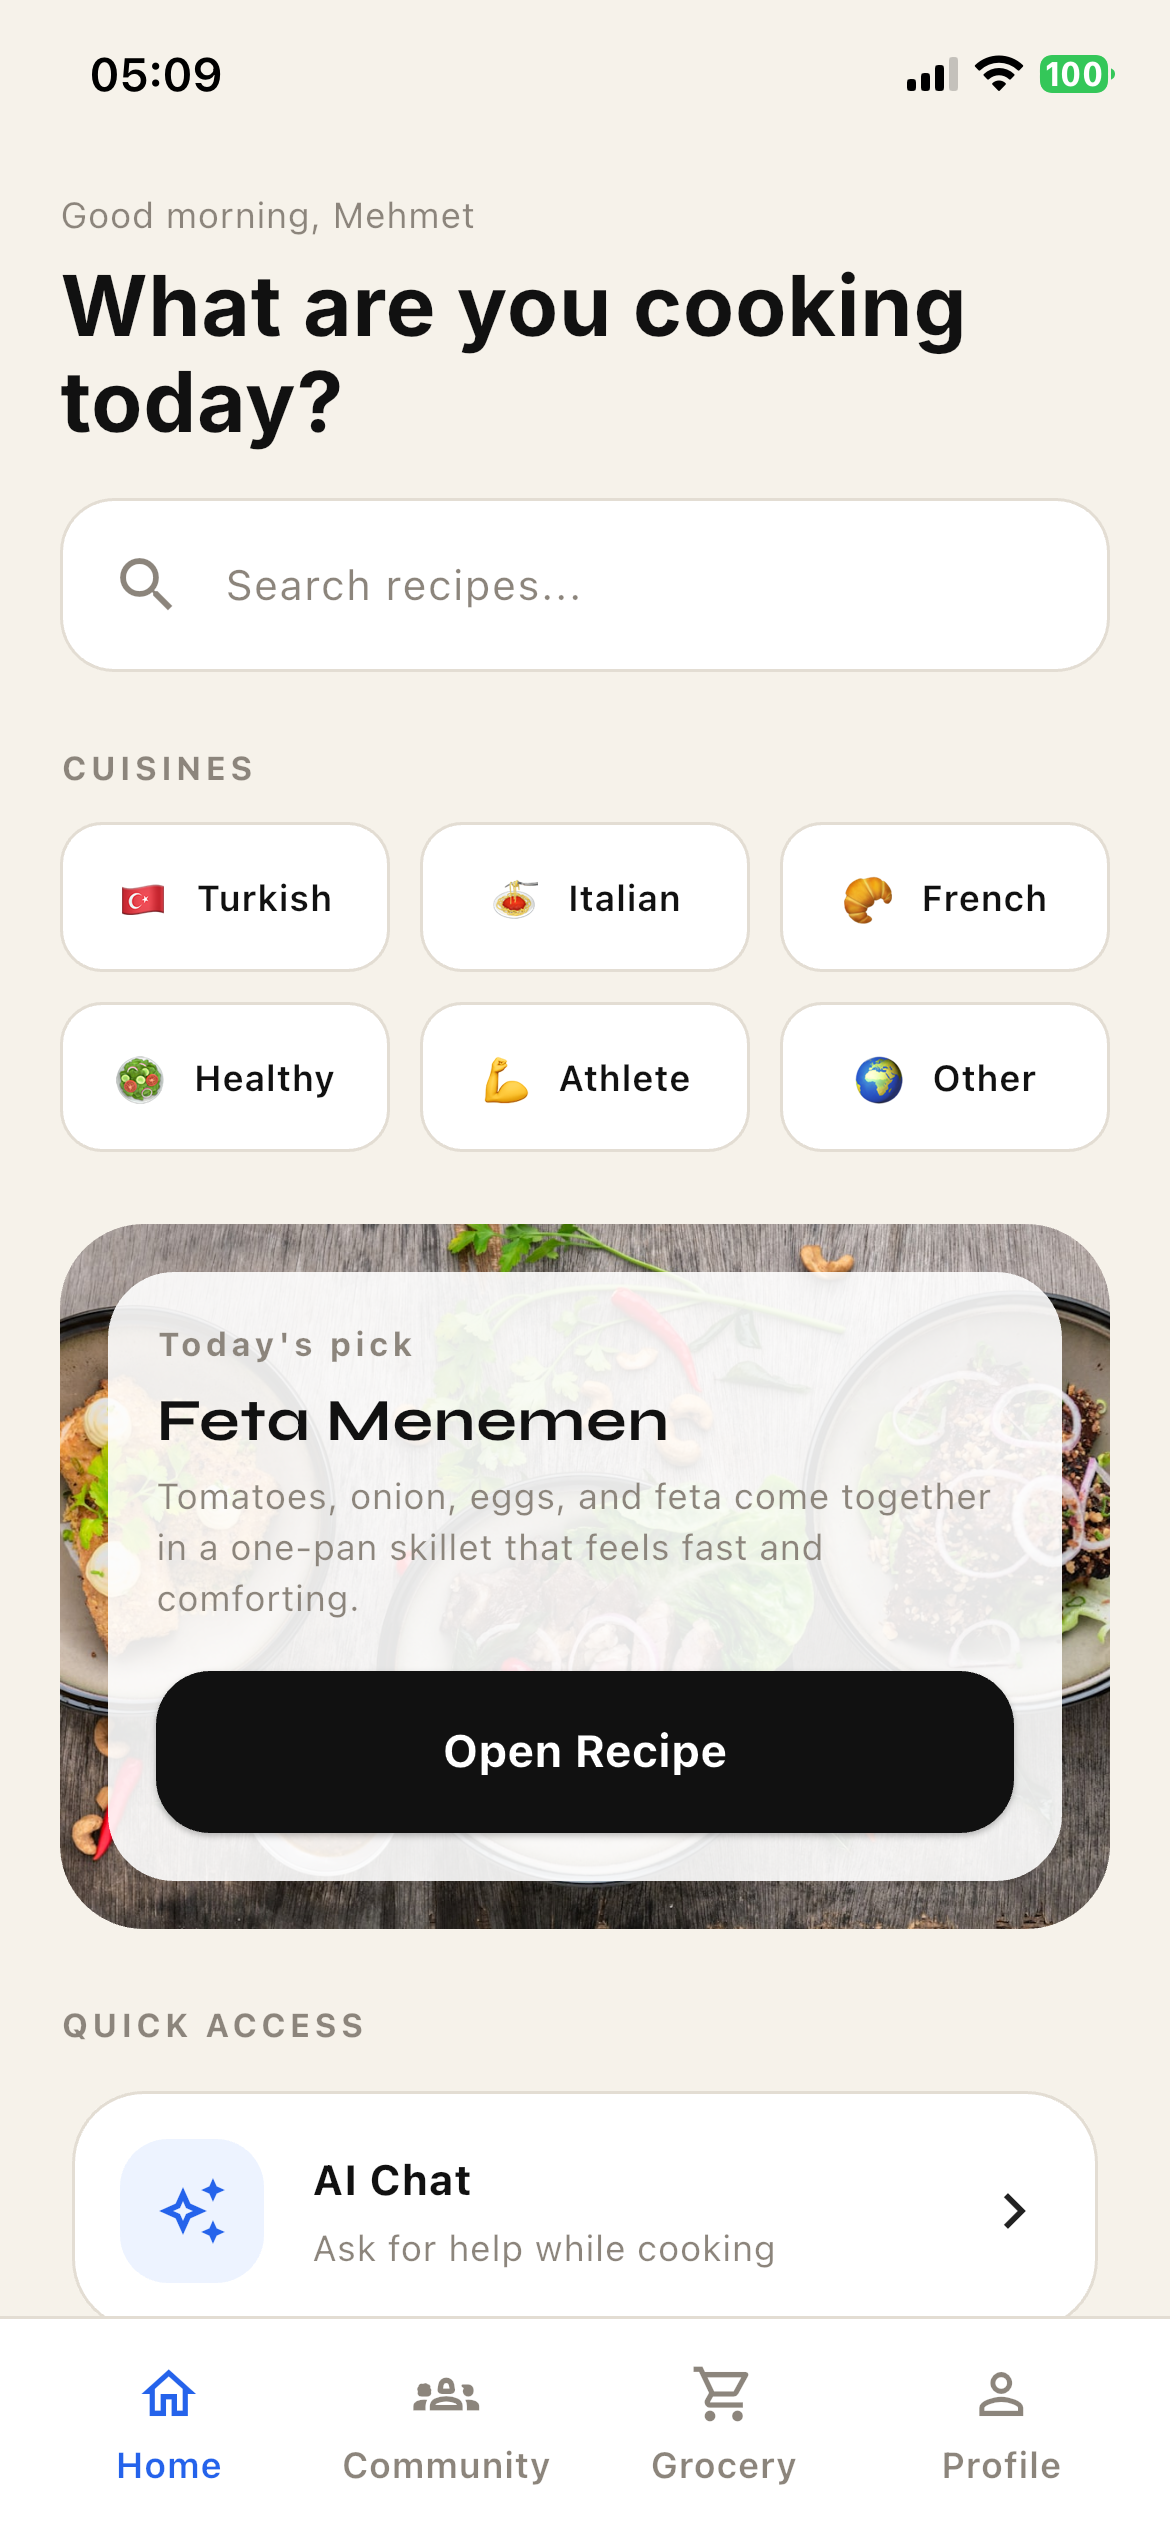
\includegraphics[width=0.80\linewidth]{screenshots/home.PNG}\\[5pt]
  {\small\bfseries Screen 4 — Home}
\end{minipage}%
\hfill
\begin{minipage}[c]{0.62\textwidth}
  The central hub of the application. Displays a personalised greeting using the logged-in user's first name (fetched from the API), a smart search bar with live autocomplete overlay, a \emph{Today's Pick} recipe card (deterministic daily rotation), a 3-column cuisine grid with emoji flags (Turkish, Italian, French, Healthy, Athlete, Other), and a Quick Access card list. The four-tab bottom navigation bar is always visible.
\end{minipage}

\medskip

%% ── 3. DISCOVERY ────────────────────────────────────────────────────────────
\subsection{Recipe Discovery Flow}

\medskip\noindent
\sblock{screenshots/cuisine.PNG}{5}{Browse Cuisine}{%
  Six cuisine tiles in a 2-column grid, each showing an emoji and label. Every tile offers two actions: \emph{Browse} (navigates directly to Recipe Results filtered by cuisine) and \emph{By pantry} (opens Ingredient Picker with the cuisine pre-set).}
\hfill
\sblock{screenshots/recipe_detail.PNG}{6}{Recipe Detail}{%
  Hero image with overlaid circular back and bookmark buttons. Displays title, tag pills (duration, servings, category), description, and three tool cards: Adjust Servings, Customize Ingredients, and Ask Chef AI. A full-width \emph{Start Cooking} button anchors the bottom.}
\hfill
\sblock{screenshots/serving_scale.PNG}{7}{Serving Scale}{%
  Stepper card with $-$ / $+$ buttons updates the serving count; the API recalculates and returns scaled ingredient quantities in real time. Each ingredient is shown as a \texttt{Card} with its name and computed amount.}

\medskip

%% ── 4. TOOLS ─────────────────────────────────────────────────────────────────
\subsection{Recipe Tools}

\medskip\noindent
\sblock{screenshots/customize_ingredients.PNG}{8}{Customize Ingredients}{%
  Grid of ingredient chips loaded from the API. Tapping a chip toggles it as a replacement target. \emph{Apply Changes} posts the selection to the backend and confirms via \texttt{AlertDialog}.}
\hfill
\sblock{screenshots/cooking_steps.PNG}{9}{Cooking Steps}{%
  All recipe steps rendered as numbered cards (coloured circle + white card). A single \emph{Mark as Done} button at the bottom triggers a completion \texttt{AlertDialog} and returns the user to Home.}
\hfill
\sblock{screenshots/ai.PNG}{10}{AI Chef Chat}{%
  Full-screen custom \texttt{Scaffold} (no shared \texttt{ChefPage} wrapper). Recipe context badge at the top. Chef replies on the left (white bubble), user messages on the right (dark bubble). \texttt{ScrollController} auto-scrolls to the latest message.}

\medskip

%% ── 5. UTILITY ───────────────────────────────────────────────────────────────
\subsection{Utility and Social Screens}

\medskip\noindent
\sblock{screenshots/grocery_list.PNG}{11}{Grocery List}{%
  Missing ingredients shown as \texttt{Card} widgets in a live list. Each card has a delete \texttt{IconButton} that calls the API and removes the item from the local \texttt{\_items} list with \texttt{setState}. An \emph{Add Items} button opens a bottom sheet with 12 quick-add chips and a free-text field.}
\hfill
\sblock{screenshots/saved_recipes.PNG}{12}{Saved Recipes}{%
  Bookmarked recipe cards fetched from the API. Each card shows the author, cover image, title, and description. Tapping the bookmark icon calls \texttt{removeSavedRecipe()} and splices the item out of the list in real time.}
\hfill
\sblock{screenshots/community.PNG}{13}{Community}{%
  Social feed of community posts loaded via \texttt{FutureBuilder}. Includes a Q\&A button (navigates to AskQAScreen) and a FAB for posting. Tapping an author avatar opens UserProfileScreen via named route.}

\medskip\noindent
\begin{minipage}[c]{0.34\textwidth}
  \centering
  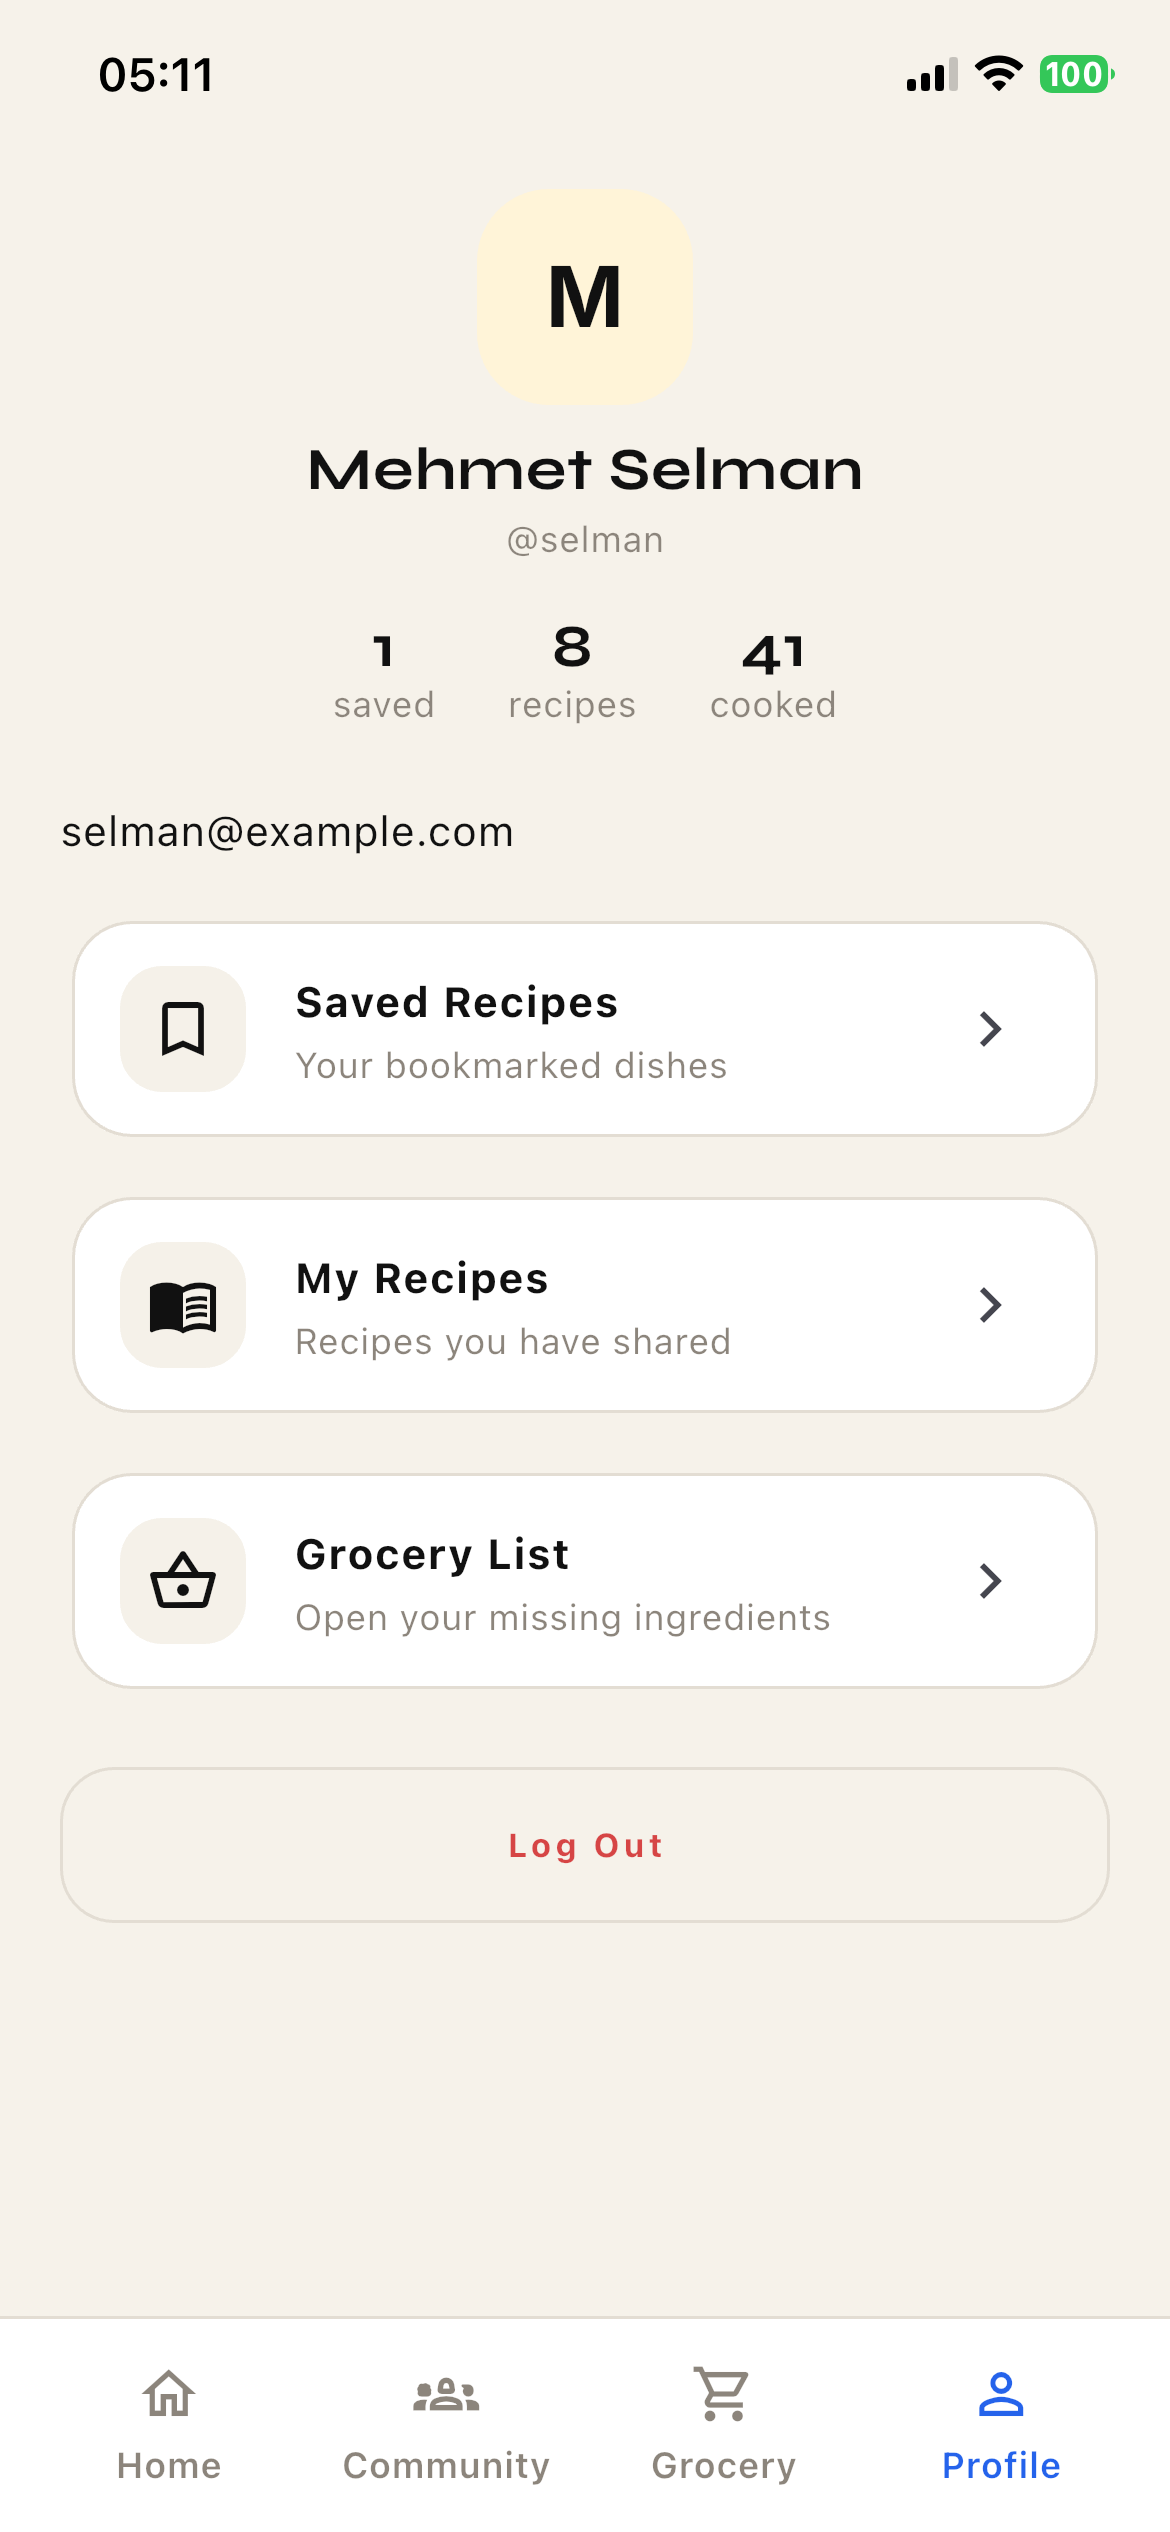
\includegraphics[width=0.80\linewidth]{screenshots/profile.PNG}\\[5pt]
  {\small\bfseries Screen 14 — Profile}
\end{minipage}%
\hfill
\begin{minipage}[c]{0.62\textwidth}
  Personal account hub loaded from the API using the stored login email. Displays stat tiles (saved recipes, published recipes, cooked meals) and a menu list (Saved Recipes, My Recipes, Post a Recipe, Adjust Servings, Customize Ingredients). A \emph{Log Out} button clears the session and returns to Onboarding.
\end{minipage}

%% ══════════════════════════════════════════════════════════════
\newpage
\section{Technical Features}

\subsection{Named Routes}

All navigation is implemented through Flutter's named route system defined in \texttt{lib/routes/app\_routes.dart}. Every route string is a \texttt{static const} field of the \texttt{AppRoutes} class, preventing typos and enabling IDE navigation. The \texttt{MaterialApp} in \texttt{lib/app.dart} declares all 20 routes in its \texttt{routes} map and sets \texttt{initialRoute: AppRoutes.onboarding}.

Navigation calls used throughout the app:
\begin{itemize}
  \item \texttt{Navigator.pushNamed(context, AppRoutes.recipeDetail, arguments: slug)} — pushes onto the stack and passes data via the \texttt{arguments} parameter. Receiving screens read it with \texttt{ModalRoute.of(context)?.settings.arguments}.
  \item \texttt{Navigator.pushReplacementNamed} — used by the bottom navigation bar to swap root screens without growing the stack.
  \item \texttt{Navigator.pushNamedAndRemoveUntil(context, AppRoutes.home, (r) => false)} — used after successful login/register and after \emph{Mark as Done} in Cooking Steps, ensuring no stale screens remain in the back stack.
\end{itemize}

\subsection{Utility Classes}

Three dedicated utility files live in \texttt{lib/utils/}, each with a private constructor so they cannot be instantiated — all members are \texttt{static} or \texttt{static const}:

\begin{itemize}
  \item \textbf{\texttt{AppColors}} — Defines the full colour palette: \texttt{primary} (warm orange-brown), \texttt{primarySoft} (tinted fill), \texttt{background} (cream \texttt{\#FAF7F2}), \texttt{border}, \texttt{textPrimary}, \texttt{textMuted}. Referenced directly as \texttt{AppColors.primary} throughout every screen and widget.
  \item \textbf{\texttt{AppTextStyles}} — Provides six \texttt{static const TextStyle} values: \texttt{display}, \texttt{title}, \texttt{subtitle}, \texttt{body}, \texttt{caption}, \texttt{sectionLabel}. Each references either the \texttt{Inter} or \texttt{Syne} font family (see Section~5.4), ensuring typographic consistency across all 20 screens.
  \item \textbf{\texttt{AppSpacing}} — Named spacing constants: \texttt{xs = 4}, \texttt{sm = 8}, \texttt{md = 16}, \texttt{lg = 24}, \texttt{xl = 32}. Used in every \texttt{SizedBox}, \texttt{Padding}, and \texttt{EdgeInsets} across the codebase.
\end{itemize}

\subsection{Asset and Network Images}

\textbf{Asset images} are stored in \texttt{assets/images/} and declared in \texttt{pubspec.yaml} under \texttt{flutter.assets}:
\begin{itemize}
  \item \texttt{onboarding-meal.jpg} — food collage shown on the Onboarding screen.
  \item \texttt{recipe-hero.jpg} — fallback hero used when a recipe has no remote image.
  \item \texttt{community-bowl.jpg} — fallback for community post cards with broken image URLs.
\end{itemize}
All three are loaded with \texttt{Image.asset('assets/images/...')} and displayed inside \texttt{ClipRRect} or \texttt{DecorationImage} widgets.

\textbf{Network images} are loaded with \texttt{Image.network(url)} for recipe cover photos sourced from Unsplash (e.g.\ \texttt{https://images.unsplash.com/photo-1504674900247-...}). Every \texttt{Image.network} call includes an \texttt{errorBuilder} callback that falls back to the corresponding asset image, preventing broken-image placeholders on network errors.

\subsection{Custom Fonts}

Two external font families are bundled with the application, declared in \texttt{pubspec.yaml} under \texttt{flutter.fonts}:
\begin{itemize}
  \item \textbf{Inter} — loaded from \texttt{assets/fonts/Inter.ttf}. Applied to \texttt{AppTextStyles.display}, \texttt{body}, \texttt{subtitle}, \texttt{caption}, and \texttt{sectionLabel}. Used for all body-level and UI text throughout the app.
  \item \textbf{Syne} — loaded from \texttt{assets/fonts/Syne.ttf}. Applied to \texttt{AppTextStyles.title}. Used for card titles and section headers, giving them a distinct geometric feel that matches the brand identity.
\end{itemize}
Both fonts are referenced only through \texttt{AppTextStyles} constants, so switching the font for the entire app requires a single file change.

\subsection{Card-Based List with Dynamic Item Removal}

Two screens demonstrate \texttt{Card} widgets rendering model-class instances with live removal:

\textbf{GroceryListScreen} (\texttt{lib/screens/grocery\_list\_screen.dart}):
\begin{itemize}
  \item Data model: \texttt{GroceryItem} (fields: \texttt{id}, \texttt{title}, \texttt{checked}) defined in \texttt{lib/models/app\_models.dart}.
  \item Each item is rendered as a \texttt{Card} containing the item title and a trailing delete \texttt{IconButton}.
  \item Pressing delete calls \texttt{ApiService.instance.removeGroceryItem(item.id)}, then updates the local \texttt{\_items} list inside \texttt{setState(() \{ \_items.removeWhere(...); \})} — the item disappears from the UI immediately with no full reload.
\end{itemize}

\textbf{SavedRecipesScreen} (\texttt{lib/screens/saved\_recipes\_screen.dart}):
\begin{itemize}
  \item Data model: \texttt{SavedRecipe} (fields: \texttt{recipeSlug}, \texttt{title}, \texttt{author}, \texttt{imageUrl}, \texttt{description}) defined in \texttt{lib/models/app\_models.dart}.
  \item Each saved recipe is a \texttt{Card} with a cover image, title, description, and a bookmark \texttt{IconButton}.
  \item Tapping the bookmark calls \texttt{ApiService.instance.removeSavedRecipe(slug)}, then removes the entry from \texttt{\_savedRecipes} with \texttt{setState}, reflecting the change instantly.
\end{itemize}

\subsection{Form Validation with AlertDialog}

\textbf{LoginScreen} (\texttt{lib/screens/login\_screen.dart}) uses a \texttt{Form} widget with a \texttt{GlobalKey\allowbreak<FormState>}:

\begin{itemize}
  \item \textbf{Email field} — \texttt{TextFormField} with \texttt{validator}: returns an error string if the value is empty or does not contain \texttt{@}. Error message: \emph{``Enter a valid email''}.
  \item \textbf{Password field} — \texttt{TextFormField} with \texttt{validator}: returns an error if empty or fewer than 6 characters. Error message: \emph{``Use at least 6 characters''}.
  \item On submit, \texttt{\_formKey.currentState!.validate()} is called first. If it returns \texttt{false}, both fields render their inline red error text below the respective input and the API call is \emph{not} made.
  \item On a successful API response, \texttt{showSuccessDialog()} is invoked, which calls \texttt{showDialog} with an \texttt{AlertDialog} containing the title \emph{Welcome Back}, a confirmation message, and a \emph{Continue} button that navigates to Home with \texttt{pushNamedAndRemoveUntil}.
\end{itemize}

\textbf{RegisterScreen} follows the same pattern with four validated fields (full name, email, password, confirm password) and its own success \texttt{AlertDialog}.

\subsection{Responsiveness}

All screens are wrapped by the shared \texttt{ChefPage} widget (\texttt{lib/widgets/common\_widgets.dart}), which implements a two-level responsiveness strategy:

\begin{enumerate}
  \item \textbf{Maximum width constraint:} Content is placed inside \texttt{ConstrainedBox(constraints: BoxConstraints(maxWidth: 620))} aligned to the top-centre of the screen. On tablets or landscape iPads, this prevents content from stretching unreadably wide, keeping a readable line length at all sizes.
  \item \textbf{Adaptive horizontal padding:} A \texttt{LayoutBuilder} reads \texttt{constraints.maxWidth}. If the screen is wider than 700 logical pixels, \texttt{horizontalPadding} is set to \texttt{40.0}; otherwise it is \texttt{20.0}. This makes the layout feel native on both phones and larger devices.
\end{enumerate}

Additionally, \texttt{IngredientPickerScreen} uses its own inner \texttt{LayoutBuilder} to switch the ingredient grid between 2 columns (narrow phones) and 4 columns (screens wider than 420px). \texttt{Wrap} widgets are used for tag chips on Recipe Detail and Browse Cuisine, so they reflow naturally at any width.

%% ══════════════════════════════════════════════════════════════
\section{UI Implementation vs.\ Wireframes}

The Flutter implementation is a faithful translation of the Step~2 wireframes with the following direct correspondences:

\begin{itemize}
  \item \textbf{Colour palette} — The warm cream background (\texttt{\#FAF7F2}), primary accent (orange-brown), white cards, and muted borders are identical to the Figma designs. All values are centralised in \texttt{AppColors}.
  \item \textbf{Typography hierarchy} — Display headings (28 px bold), section titles (20 px Syne), muted subtitles, and small captions map directly to the wireframe text hierarchy. Inter is used for all body text as specified in the design system.
  \item \textbf{Bottom navigation} — Four tabs (Home, Community, Grocery, Profile) with icon + label, active item highlighted in primary colour — exactly as designed.
  \item \textbf{Card language} — All recipe cards, tool cards, and profile menu items use 20--28 px rounded rectangles with a 1 px border and white fill, matching the wireframe card components.
  \item \textbf{Cuisine grid} — The wireframe's 3-column emoji grid is reproduced with a fixed \texttt{childAspectRatio: 2.2} for the horizontal pill shape, matching the compact tile style.
  \item \textbf{Recipe Detail hero} — Overlaid circular back button (top-left) and bookmark button (top-right) on a 16:10 aspect-ratio image, as shown in the wireframe.
  \item \textbf{AI Chat layout} — Full-screen scaffold with a fixed header, scrollable message list, and a pinned input bar at the bottom — reproducing the wireframe chat layout exactly.
  \item \textbf{Additions beyond wireframes} — Smart search autocomplete on Home, round back buttons on all sub-screens, and a Today's Pick recipe card were added to improve usability while keeping the overall visual language consistent.
\end{itemize}

\end{document}
